\section{Versuchsauswertung}

\subsection{Solarstrahlung} 

\subsubsection{Aufnahme der Messdaten}
Zur Bestimmung der Solarstrahlung wurden folgende Halbleitersensoren und Pyranometern in die Messdatenerfassung eingebunden:

\begin{center}
	
\begin{tabular}{l|l}	
	\label{tab:Sensoren}
	\textbf{Sensorname} & \textbf{Sensorart}\\
	\hline
	CM 11 & Thermosäule\\
	CM 11 (mit Schattenring) & Thermosäule\\
	CM3 & Thermosäule\\
	SSR 81 & Halbleiter\\
	TA GBS & Halbleiter
\end{tabular}
\end{center}

Der Schattenring des Pyranometers zur Messung der Diffusstrahlung wurde nach Tabelle 5 des Praktikumsskriptes ausgerichtet. Die Ausrichtung der Messtafel mit den übrigen Sensoren Richtung Sonne konnte nur geschätzt werden, da der Himmel zum Zeitpunkt der Messung bedeckt war. Für die weitere Auswertung wird daher ein bereitgestellter Datensatz (vgl. Abbildung \ref{fig:radiation}) verwendet.

\begin{figure}[H]
	\centering
	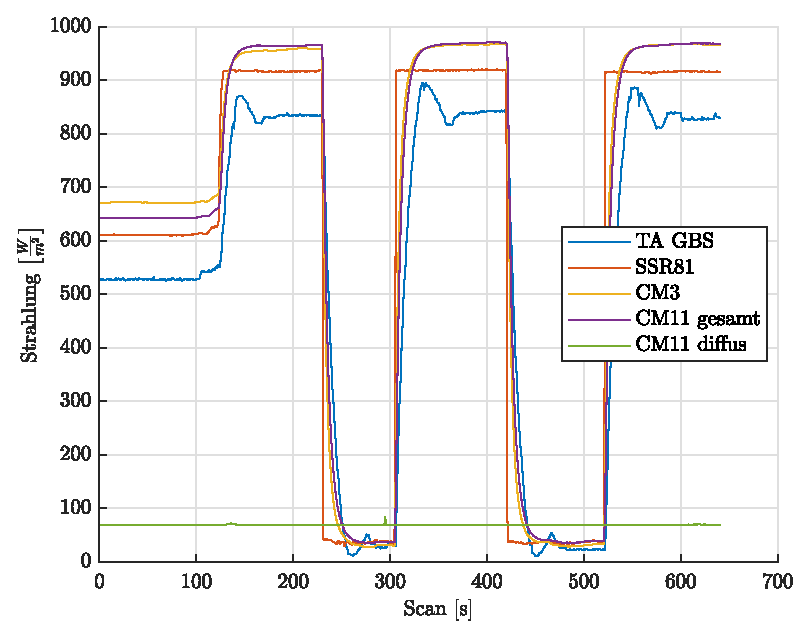
\includegraphics[width=0.8\textwidth]{../DATA/Messreihe_Strahlung.eps}
	\caption[Messreihe zur Bestimmung der Solarstrahlung]{Messreihe zur Bestimmung der Solarstrahlung}
	\label{fig:radiation}
\end{figure}
Zum Vergleich der Messwerte wurden der Mittelwert und die Standardabweichung der einzelnen Sensoren über den stationären Messbereich zwischen Sekunde 170 und Sekunde 220 gebildet. Tabelle \ref{tab:radiation} zeigt die bestimmten Werte.
\begin{center}
\begin{tabular}{l|c|c}
	\label{tab:radiation}
	
	\textbf{Sensor} & \textbf{Strahlung [$\frac{W}{m^2}$]} & \textbf{Standardabweichung}\\
	\hline
	TA GBS & 833,6252 & 2,1081\\
	SSR81 & 916,4836 & 0,6581\\
	CM3 & 957,7781 & 1,7451\\
	CM11 & 964,5125 & 0,4149\\
	CM11 (diffus) & 68,6927 & 0,1916
\end{tabular} 
\end{center}

Die Angegeben Strahlungswerte beziehen sich auf die Globalstrahlung. Das mit einem Schattenring ausgestattete CM11 Pyranometer misst hingegen nur die Diffusstrahlung. Die Direktstrahlung kann mittels folgender Gleichung aus den beiden CM11 Pyranometern berechnet werden:
\begin{equation}
	\label{eq:Edir}
	E_{dir}=E_{global}-E_{diffus}=\SI{964.5125}{\watt\per\square\meter}-\SI{68.692}{\watt\per\square\meter} = \SI{895.8205}{\watt\per\square\meter}
\end{equation}

Aus dem Datensatz geht hervor, dass die Halbleitersensoren verglichen mit den Pyranometern eine geringere Strahlung messen. Der induzierte Photoeffekt ist bei Halbleitersensoren abhängig von der Wellenlänge. Aufgrund dieser Verluste wird ein niedrigere Ausgangsspannung am Messwiderstand gemessen. Für eine genauere Messung müsste der Sensor anhand einer definierten Strahlungsleistung (Bsp. Sonnensimulator) kalibriert werden. Weiterhin sind die verwendeten Halbleitersensoren nach keinem Standard klassifiziert, sodass keine nähere Aussage über die messgenauigkeit getroffen werden kann. Thermosäulen liefern präzisere Messwerte, da sie ein Thermisches Messverfahren nutzen und Verluste durch den Glasdom gemindert werden. Die verwendeten CM11 Pyranometer sind nach dem Secondary Standard klassifiziert und sollten daher im Rahmen des Versuchs als Referenz betrachtet werden.


\subsubsection{Bestimmung des Ansprechverhaltens}
Wie im vorherigen Teil der Auswertung wurden bereitgestellte Daten verwendet. Die Messreihe ist in Abbildung \ref{fig:response} gezeigt.
\begin{figure}[H]
	\centering
	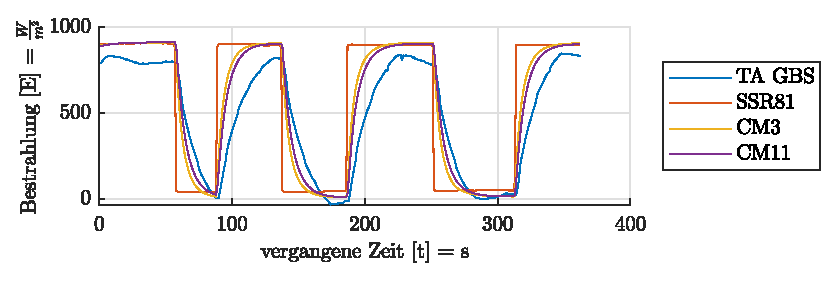
\includegraphics[width=0.8\textwidth]{../DATA/Messreihe_Ansprechzeit.eps}
	\caption[Messreihe zur Bestimmung des Ansprechverhaltens.]{Messreihe zur Bestimmung des Ansprechverhaltens.}
	\label{fig:response}
\end{figure}

\subsection{Luftfeuchtemessung}
Zunächst wurden die Umgebungstemperatur und die Ausgangsspannung des Feuchtesensors ermittelt. Abbildung \ref{fig:amb} zeigt den Messverlauf. Die Mittelwerte und Standardabweichungen sind in Tabelle \ref{tab:amb} zusammengefasst.

\begin{figure}[H]
	\centering
	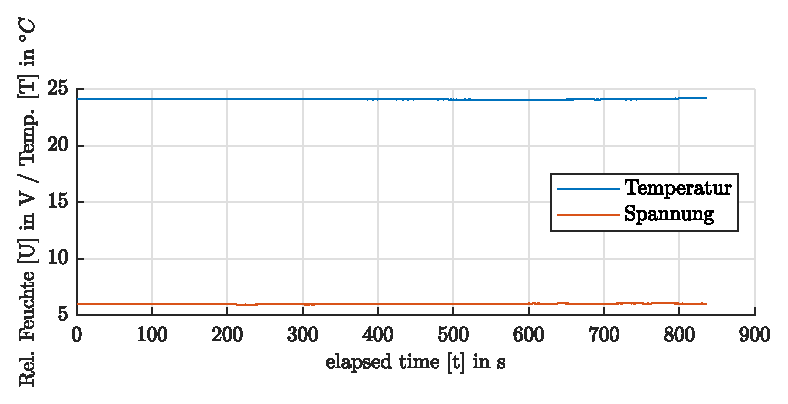
\includegraphics[width=0.8\textwidth]{../DATA/Messreihe_Umgebung.eps}
	\caption[Messreihe Umgebung]{Messreihe zur Bestimmung der Umgebungstemperatur und -luftfeuchte.}
	\label{fig:amb}
\end{figure}

\begin{center}
	\begin{tabular}{l|c|c}
		\label{tab:amb}
		
		\textbf{Messgröße} & \textbf{Mittelwerte} & \textbf{Standardabweichung}\\
		\hline
		Umgebungstemperatur & \SI{24,1005}{\celsius} & 0,0434\\
		Umgebungsluftfeuchte & 5,9791\,V & 0,0284
	\end{tabular}
\end{center}

Zur Bestimmung der relativen Feuchte wurde eine Kalibriergerade anhand zweier Messpunkte angefertigt. Hierzu wurde die Ausgangsspannung des Sensors zunächst über einer NaCl-Lösung, anschließend über einer LiCl-Lösung gemessen. Der Messverlauf ist in Abbildung \ref{fig:cal} aufgetragen. Es wurden jeweils die letzten 100 Scans zur Bestimmung der Ausgangsspannung gemittelt (vgl. Tabelle \ref{tab:cal}). Bei der vorliegenden Umgebungstemperatur von ca. \SI{24}{\celsius} entspricht die relative Luftfeuchte über NaCl 75\,\%, über LiCl 12\,\%. 

\begin{figure}[H]
	\centering
	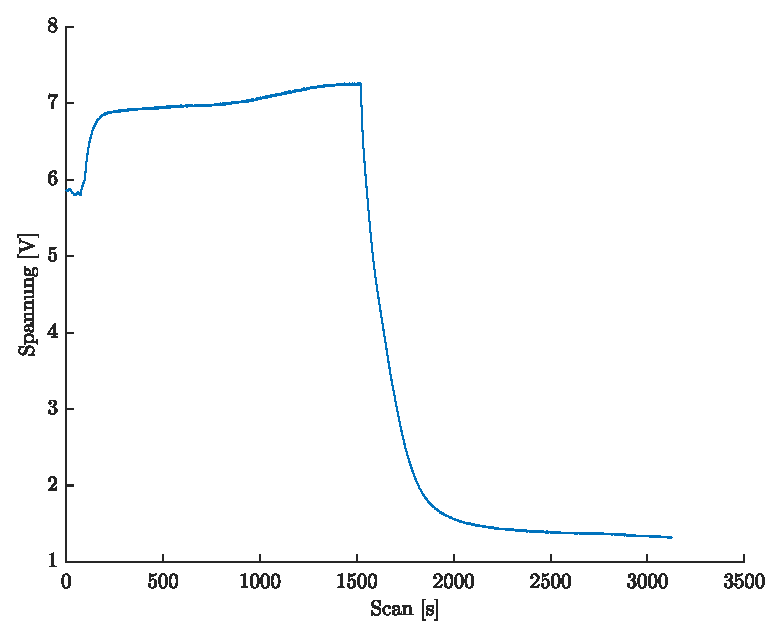
\includegraphics[width=0.8\textwidth]{../DATA/Messreihe_Feuchtekalibration.eps}
	\caption[Kalibrationsmessung]{Kalibrationsmessung anhand zweier Salzlösungen. Zum Zeitpunkt t=1500s wurde der Sensor von der NaCl-Lösung über die LiCl-Lösung überführt.}
	\label{fig:cal}
\end{figure}

Aus Abbildung \ref{fig:cal} geht hervor, dass die Spannungen nicht konstant gemessen wurden. Für eine genauere Kalibration ist eine längere Verweilzeit über den Salzlösungen nötig. Prinzipiell eignen sich die gewählten Messpunkte gut, da die Luftfeuchte über den verwendeten Lösungen nahezu temperaturunabhängig ist. Die Messkurve des Sensors wird im Versuch als linear betrachtet, über den wahren Verlauf kann keine Aussage getroffen werden. Zur Optimierung müssen daher weitere Messpunkte aufgenommen werden.
\begin{center}
	\begin{tabular}{l|c|c|c}
		\label{tab:cal}
		
		\textbf{Kalibrierlösung} & \textbf{Mittelwerte} [V]& \textbf{Standardabweichung} & rel. Feuchte [\%]\\
		\hline
		LiCl & 1,3298 & 0,0052 & 12\\
		NaCl & 7,2433 & 0,0056 & 75
	\end{tabular}
\end{center}

Die Kalibriergerade (vgl. Abbildung \ref{fig:cal2}) wurde anhand der Spannungen aus Tabelle \ref{tab:cal} erstellt. Diese wird als Polynom erster Ordnung beschrieben (vgl. Gleichung \ref{eq:pol}).
\begin{equation}
	\label{eq:pol}
	\varphi(\text{V}) = p1*\text{V} + p2
\end{equation}

\begin{figure}[H]
	\centering
	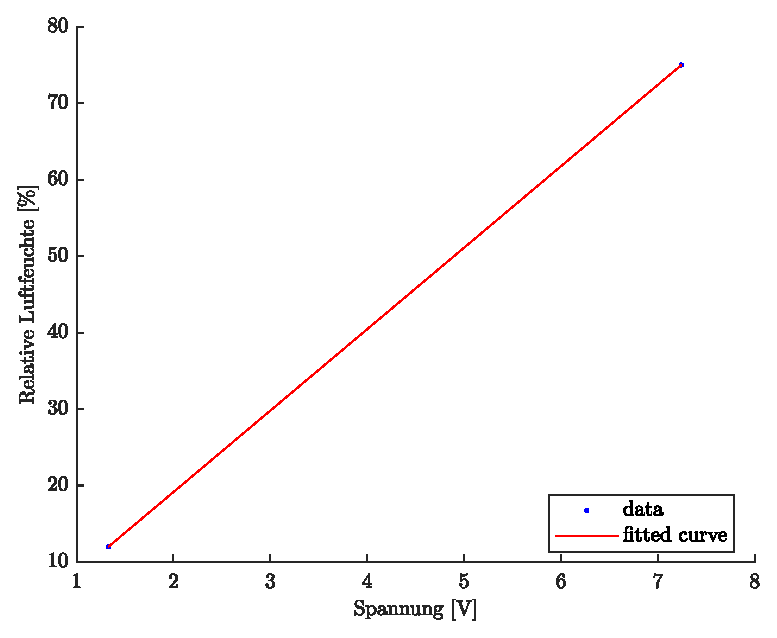
\includegraphics[width=0.8\textwidth]{../DATA/Kalibriergerade_Feuchte.eps}
	\caption[Kalibrationsgerade des Temperatursensors]{Kalibrationsgerade des Temperatursensors mit der Fit-Funktion $f(x) = p1*x + p2$ und den Parametern p1=10,65 und p2=0.2034}
	\label{fig:cal2}
\end{figure}

Die relative Feuchte der Umgebungsluft errechnet sich nach Abbildung \ref{fig:cal2} und Gleichung \ref{eq:pol} zu

\begin{equation}
	\label{eq:cal}
	\varphi(\text{V})=10,65*\SI{5,9791}{\volt}-2,167=\SI{61,51}{\percent}
\end{equation}
		
\subsection{Niederschlag}
Zur Simulation des Niederschlags wurde in drei Durchläufen je \SI{1}{\liter} Wasser in den Auffangtrichter gegossen und die Impulse der Messwippe gezählt. Abbildung \ref{fig:rain} zeigt die aufgenommenen Messdaten. 

\begin{figure}[H]
	\centering
	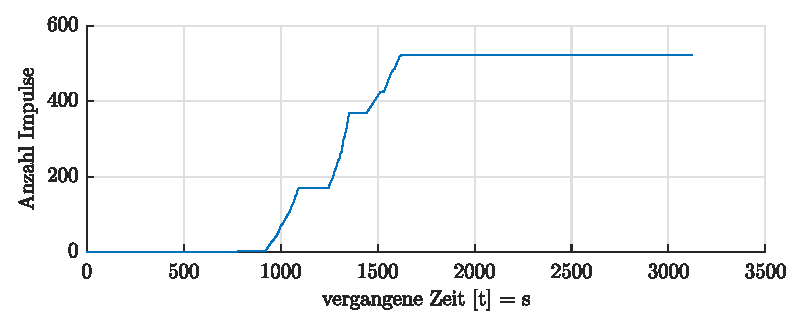
\includegraphics[width=0.8\textwidth]{../DATA/Messreihe_Niederschlag.eps}
	\caption[Datenerfassung zur Niederschlagsbestimmung]{Datenerfassung zur Niederschlagsbestimmung.}
	\label{fig:cal2}
\end{figure}

Die Impulszahl entspricht jeweils der Differenz des Ordinatenabschnittes zwischen den Messungen. Zusätzlich wurde die Messdauer betrachtet und der Volumenstrom bilanziell aus dem Kehrwert der Messdauer berechnet. Das Volumen der Wippen wurde aus dem Kehrwert der Impulszahl berechnet (vgl. Tabelle \ref{tab:rain}).

 \begin{center}
 	\begin{tabular}{c|c|c|c|c}
 		\label{tab:rain}
 		\textbf{Messung} & \textbf{Impulszahl} & \textbf{Messdauer} [s] & \textbf{Volumenstrom} [$\frac{ml}{s}$] & \textbf{Liter pro impuls}\\
 		\hline
 		1 & 166 & 168 & 5,95 & 6,02\\
 		2 & 200 & 105 & 9,52 & 5,00\\
 		3 & 153 & 171 & 5,85 & 6,54\\
 		Mittel & 173 & 148 & 7,11 & 5,85
 	\end{tabular}
 \end{center}

Das Messergebnis ist in erster Linie vom zufließenden Volumenstrom abhängig. Bei geringerem Zufluss wird Wippe  langsam an ihren Kipppunkt gebracht, während sie bei höheren Zuflussraten durch den Impuls des Fluids schon vor der vollständigen Befüllung kippt. Dieser Trend ist in Tabelle \ref{tab:rain} zu sehen. Das Volumen pro Impuls ist bei Messung 2 am geringsten, der bilanzielle Volumenstrom am größten. Die Messmethode ist daher tendenziell für die Messung bei leichten Regenschauern geeignet. Bei Starkregen versagt sie.

Für die Bestimmung der Niederschlagshöhe wird zunächst nach Gleichung \ref{eq:rain} die Tricherfläche bestimmt:

\begin{equation}
	\label{eq:rain}
	A= \pi * r^2= \pi * (\frac{\SI{0,165}{\meter}}{2})^2 = \SI{0,0214}{\square\meter}
\end{equation}

Die normierte Niederschlagshöhe ergibt sich entsprechend Gleichung \ref{eq:rain2} aus dem Quotienten der Niederschlagsmenge und der Trichterfläche:

\begin{equation}
	\label{eq:rain2}
	h = \frac{V}{A} = \frac{\SI{0,001}{\cubic\meter}}{\SI{0,0214}{\square\meter}} = \SI{0,0467}{\meter} = \SI{46,7}{\milli\meter}
\end{equation}

\subsection{Windmessung}
Eine sinnvolle Messung der Luftströmung war aufgrund der ungünstigen Position der Messstation nicht möglich. Daher wird auch bei diesem Versuchsteil auf einen bereitgestellten Dtensatz zurückgegriffen.

\subsubsection{Windrichtung}